% Pipeline


feature extractors are nb bc they r iinvariant to scale rotation and transformation. As opposed to simply correlating entire image. also less computationally expensive.
https://baotramduong.medium.com/feature-extraction-in-computer-vision-using-python-358d7c9863cb




General selection criteria:

\begin{itemize}
    \item \textbf{Accuracy}: The method should provide accurate results, judged by the error passed down the pipeline. 
    \item \textbf{Speed}: Real-time applications require fast, scalable processing, judged by their entire effect on the pipeline runtime.
    \item \textbf{Price}: The method should be free. This excludes popular detectors like SIFT and SURF, which require licensing fees.
    \item \textbf{Robustness}: The methods should be invariant to changes in scale, rotation, illumination, and noise to ensure reliable performance across varied environments. Further, the method should ensure repeatability. 
\end{itemize}





\section*{Feature Detectors} 

%https://mikhail-kennerley.medium.com/a-comparison-of-sift-surf-and-orb-on-opencv-59119b9ec3d0


Feature extraction plays a vital role in image-based UAV navigation, where estimating transformations such as rotation and translation between consecutive images is crucial. Feature extractors detect keypoints—distinct, repeatable points in an image—and generate descriptors that encode information about the surrounding region. These keypoints and descriptors enable accurate matching across multiple frames, allowing the system to track movement while remaining invariant to changes in scale, rotation, and illumination. This process enables precise estimation of motion, including both rotational and translational shifts between images.


\subsection*{Types of Feature Extractors}

\subsubsection{ORB (Oriented FAST and Rotated BRIEF)}
ORB consists of two main components: the FAST keypoint detector and the BRIEF descriptor. FAST (Features from Accelerated Segment Test) detects keypoints by examining a circular region of pixels around a candidate point and checking whether a segment of these pixels is significantly brighter or darker than the center. This allows ORB to quickly identify potential keypoints. Once detected, BRIEF (Binary Robust Independent Elementary Features) describes these keypoints by creating a binary string, where pixel intensity comparisons within a small patch around each keypoint are encoded. ORB also adds rotational invariance by aligning the keypoints based on their dominant orientation before computing the BRIEF descriptor. This process ensures that ORB is fast and invariant to scale and in-plane rotation, though it may struggle with repetitive textures or complex lighting changes.

\subsubsection*{AKAZE (Accelerated-KAZE)}
AKAZE operates by constructing a nonlinear scale space using efficient filtering based on diffusion processes. This nonlinear scale space captures fine image details more effectively than linear methods. AKAZE computes the local contrast of an image using a specialized filter that adapts to intensity variations, allowing it to detect subtle keypoints that simpler detectors might miss. Once keypoints are detected, AKAZE uses the Modified Local Difference Binary (MLDB) descriptor, which encodes the neighborhood of each keypoint into a binary vector by comparing pixel intensity differences in the region. This approach is fast and compact, but AKAZE’s sensitivity to its detection threshold can vary across environments, leading to inconsistent keypoint detection. To address this, dynamic thresholding is applied, adjusting the threshold based on the environment to maintain a consistent number of keypoints across different datasets, improving generalization.

\subsubsection*{SuperPoint with LightGlue}
SuperPoint is a deep learning-based keypoint detector and descriptor. It uses a convolutional neural network (CNN) to detect keypoints and generate descriptors in a single forward pass. The network is pre-trained on large image datasets, learning to recognize stable and distinctive keypoints across a variety of conditions. However, being pre-trained, it may not generalize well to datasets that differ significantly from its training set. SuperPoint pairs best with LightGlue, a machine-learning-based matcher that improves matching accuracy using deep learning techniques. LightGlue optimizes keypoint correspondences between images through advanced graph-based techniques, ensuring accurate matches, even in challenging conditions. The primary downside of SuperPoint and LightGlue is computational expense, making them slower than traditional methods unless GPU acceleration is utilized. LightGlue was tested with SuperPoint during the detector testing phase and was not retested during the matcher testing phase.



\subsection*{Application}

Feature detectors were applied at four distinct stages in the UAV image-processing pipeline. Each stage addressed a specific need in the transformation estimation process. Different stages required different levels of precision and accuracy. The goal of the detector phase was to identify the efficiency and accuracy of each detector, and apply them accordingly to the subsequent stages.

For this reason there were the following tests conducted
efficiency
accuracy and robustness + generalizability - for BOTH rotation and translation estimations isolated via pass through to error. 




In the first stage, rotation between images was estimated to align them for similarity comparisons. While accuracy was necessary, runtime efficiency took priority due to the volume of image comparisons involved. Small rotational errors were acceptable, as global matchers, as tested later, showed tolerance to rotational inaccuracies. Thus, precise testing was not necessary. ORB with 6000 keypoints was chosen for this stage due to its efficiency and reasonable accuracy.

In the second stage, the goal was to use matches between images to estimate global context image similarity, focusing on the number of similar matches across grid extractions. Precision was less important here, but efficiency was paramount. ORB with 1500 keypoints was employed for this purpose. This stage’s efficiency in global similarity comparison was validated in the global matching section.

The first two stages were not explicitly tested for detector choice, as their performance largely depended on efficiency, where ORB clearly outperformed others. The focus in testing was on the latter two stages, which required higher precision.

In the third stage, accurate rotational estimation was prioritized to ensure proper alignment for translation estimation and heading output. 

In the fourth stage, precise translation estimation was needed for GPS inference. High accuracy was essential, as this stage directly affected the accuracy of positional data.

Empirical tests showed that the detector and corresponding parameter set that yielded the best translational estimate is not necessarily the best for rotational estimation. Different detectors prioritize different feature types, e.g. edges, that may suit one transformation more than another. Further, different transformations may handle the balance between number and quality of keypoints differently. Ultimately, the detector type and detection threshold must be independently found for rotational and translational estimates. 

It is for this reason tests must be conducted to find the optimal detector and parameters therefor in terms of accuracy, robustness and runtime for both rotation and translation estimation.



\subsection*{Application}
Feature detectors are used in four stages. The first is to find the rotation between images to align them for subsequent image similarity comparison. The second, is in the case when a local retrofit is used to find image similarity on a global context. The third, to find the accurate rotation change. The fourth, the accurate translation change. 
The first stage requires that rotation is calculated between the image to which inference is being done, and every reference image in the search space. As seen in the global matcher sections, these global techniques are invariant to small errors in rotational estimation. Since we are comparing multiple images, and rotational accuracy is not crucial, there is some ability to prioritize efficiency over accuracy. For this reason ORB is chosen due to its efficiency. ORB is used with 6000 keypoints. 
In the second, the matches need not be accurate, as a rough idea of the amount of matches that correspond is essential and no susbsequent inference is needed. A very crude ORB matches is used with a target of 1500 keypoints.
The third and fourth stage require accurate estimation of rotation and translation. Upon empirical testing, it was found that the detector that subtended the optimal point cloud for one piece of the transformation, did not always subtended the optimal detector for the other. Specifically, the best detector for rotation was also that for translation and vice versa. This is shown in appendix table \ref{tab:rot_reestimation}. AKAZE was shown as above to be the best for pure translation estimation and therefore dynamic keypoint target AKAZE with 3000 keypoints was chosen since the single image comparison does not require as much runtime prioritization. Since ORB performs better for the rotation estimate in general as seen in the table below, it is used. 


proof that the best detector for rotation is not also the best for translation.
TABLE:
\begin{table}[H]
    \centering
    \caption{RMSE and Runtime Comparison}
    \label{tab:rot_reestimation}
    \begin{tabular}{|c|c|c|}
    \hline
    \textbf{Dataset} & \textbf{RMSE (m)} & \textbf{Runtime (s)} \\ \hline
    \multicolumn{3}{|c|}{\textbf{WITH REESTIMATION OF ROTATION}} \\ \hline
    DATSETROT       & 67.7480           & 132.97               \\ \hline
    DATSETCPT       & 7.0124            & 131.52               \\ \hline
    DATSETROCK      & 24.6322           & 104.86               \\ \hline
    DATSETSAND      & 35.1589           & 107.22               \\ \hline
    DATSETAMAZ      & 37.3642           & 93.88                \\ \hline
    \multicolumn{3}{|c|}{\textbf{WITHOUT REESTIMATION OF ROTATION}} \\ \hline
    DATSETROT       & 68.0951           & 120.57               \\ \hline
    DATSETCPT       & 8.6607            & 100.08               \\ \hline
    DATSETROCK      & 23.2621           & 102.23               \\ \hline
    DATSETSAND      & 31.9800           & 91.50                \\ \hline
    DATSETAMAZ      & 40.0016           & 84.02                \\ \hline
    \end{tabular}
    \end{table}
    



\section*{Feature Matching}
Feature matching identifies correspondences between keypoints across images. After matching, these correspondences are filtered to remove ambiguities, and the remaining reliable matches are used to estimate transformations such as translation and rotation. Local feature matching, unlike global methods, focuses on matching individual keypoints, and not the entire image context, to achieve noise-invariant geometric transformations between images.
Each matcher outputs a list of potential matches, along with their similarity scores, represented by a descriptor-space distance metric.


\subsection*{Types Of Feature Matchers}


\begin{itemize}
    \item \textbf{Brute-Force Matcher (BFMatcher):}  
    The BFMatcher compares each feature in one image with every feature in the second image. While it guarantees the best match, it is computationally expensive.

    \item \textbf{Fast Library for Approximate Nearest Neighbors (FLANN):}  
    FLANN speeds up nearest neighbor search in high-dimensional descriptor space using KD-trees or clustering. It offers fast, approximate matching with minimal accuracy loss, ideal for real-time use with large datasets.

    \item \textbf{LightGlue:}  
    LightGlue is a machine-learning-based matcher that improves matching accuracy through deep learning. Although highly effective, it is computationally expensive. It is tested alongside SuperPoint in the feature extraction chapter, as its true potential is only realized when paired with neural network-based feature extractors. 
\end{itemize}

\subsection*{Search Techniques}
The search technique determines which potential matches are retained. Techniques such as radius matching, vanilla matching, and KNN-based matching are explored. This stage allows the matcher to control the number and quality of matches passed for further filtering.

\begin{itemize}
    \item \textbf{Radius Search:}  
    Radius search retains matches within a specified distance in descriptor space, filtering out weak matches. However, it doesn't ensure a fixed number of matches per keypoint, leading to inconsistent results. Due to this limitation, it was not used in further experiments.

    \item \textbf{Vanilla Matching:}  
    Returns the single best match for each keypoint. Empirical testing showed that this approach provided poor accuracy due to its inability to remove ambiguity with further processing. It was not further investigated.

    \item \textbf{K-Nearest Neighbors (KNN):}  
    Retains the top \textit{K} matches for each keypoint, allowing the use of post-filtering techniques like Lowe’s ratio test to remove ambiguous matches. Matches with only one neighbor were discarded to avoid compromising accuracy when Lowe’s ratio could not be applied. Empirical tests showed that values above \textit{K=2} introduced impractical computational overheads. This method was used for further experiments with \textit{K=2}.
\end{itemize}

\subsection*{Optimization Techniques}
\begin{itemize}
    \item \textbf{Lowe’s Ratio Test:}  
    Filters matches based on the ratio between the best match’s distance and the second-best match’s distance. If the ratio is below a given threshold, in other words, the matches are sufficiently different, the match is retained. While effective at removing ambiguity, Lowe’s ratio is moderately sensitive to datasets and parameters. A dynamic threshold was implemented, adjusting iteratively until a sufficient number of matches were retained while keeping iterations to a minimum.

    \item \textbf{Cross-Check:}  
    Filters matches by retaining only those that are mutual in both matching directions. This ensures that matches are one-to-one, as is often not the case due to imperfections in the dataset, reducing false positives.

    \item \textbf{RANSAC:}  
    Filters outliers by estimating transformations between images using the Random Sample Consensus (RANSAC) algorithm. It is more closely tied to the rotational and translational estimation stages, where it is tested further.

    \item \textbf{Confidence Thresholding or Weighting:}  
    Matches were filtered based on their confidence scores, determined by similarity in descriptor space. However, confidence-based filtering proved extremely sensitive to changes in parameters and datasets, limiting its applicability. This method was not further pursued.
\end{itemize}



\section*{Rotational Estimators}

Rotational estimators are crucial for aligning UAV-captured images when GPS data is unreliable. Accurate rotation alignment directly affects the estimation of translational shifts and image similarity, both of which are sensitive to small rotational errors. By determining the angular difference between consecutive images, the UAV's heading relative to a known reference point can be inferred. Since reference images have fixed headings, adjustments for Earth's curvature are unnecessary.

Three rotational estimation methods were selected for their balance between computational efficiency and accuracy. Other methods, such as direct rigid transformation via SVD, were excluded due to poor performance or outlier rejection in empirical tests. The following methods use OpenCV and RANSAC for robust estimation:

\begin{itemize}
    \item \textbf{Homography Estimation (3x3 matrix)}: 
    Homography supports 8 DoF, including translation, rotation, scaling, shear, and perspective distortion. However, in this application, the added complexity from scaling and perspective effects introduces unnecessary error. Since these transformations are not relevant to the dataset, homography is less efficient in this context.

    \item \textbf{Affine Estimation (2x3 matrix)}:
    Affine transformation provides 6 DoF: translation, rotation, scaling, and shear. It efficiently handles rotation and translation, which are the primary transformations in the dataset, without adding unnecessary complexity from perspective effects. Affine estimation strikes a good balance between accuracy and computational speed.

    \item \textbf{Partial Affine Transformation (2x3 matrix)}:
    Partial affine estimation allows for translation and rotation, providing 3 DoF. It is a simplified model, ideal for cases where minor scaling or shearing is irrelevant. This method offers a compromise between the complexity of affine transformations and the limitations of rigid transformations, providing accuracy with computational efficiency.
\end{itemize}



    
\subsection*{Rotational Normalization Strategies}

Rotational normalization is essential for aligning images and translating estimations accurately in image-based UAV navigation systems. Two primary strategies were considered for normalizing rotations during the flight back to the base. The first involves applying rotational normalization during image capture, which aligns both images to a global North-East (NE) reference space before keypoint detection. The second method avoids normalization at the point of capture, aligning the images relative to one another and applying normalization only after translation estimation.

The key difference between these two methods lies in their respective losses caused by image rotation, due to the fixed canvas size during normalization. When an image is rotated, parts of the image are lost or moved off-canvas, particularly as the rotation approaches 90 degrees (a loss of 43.75\% for an aspect ratio of 16:9). This introduces information loss, which negatively impacts the accuracy of keypoint detection and translation estimation.

The loss function for the first approach, where images are normalized independently, is proportional to:

\begin{equation}
\text{Loss}_{\text{pre}} \propto |\sin(|\Delta_1|) + \sin(|\Delta_2|)|
\end{equation}

where \( \Delta_1 \) and \( \Delta_2 \) are the respective rotation angles of the two images relative to the global coordinate system. This results in compounded losses, as both images are treated independently. The maximum loss occurs when both images are rotated by ±90 degrees, at which point the sum of sine values peaks, leading to maximum information loss.

In the second approach, where images are aligned relative to each other before normalization is applied, the loss function is:

\begin{equation}
\text{Loss}_{\text{post}} \propto |\sin(|\Delta_2 - \Delta_1|)|
\end{equation}


Here, the loss depends on the relative difference in rotation between the two images, reducing the potential for compounded information loss. In the given application, during the return flight to base, the UAV will generally undergo a near 180-degree rotation relative to the outbound path with an expected tolerance of ±20 degrees. Given this constraint, the loss functions of both approaches are as follows for various rotation scenarios:

\begin{figure}[H]
    \centering
    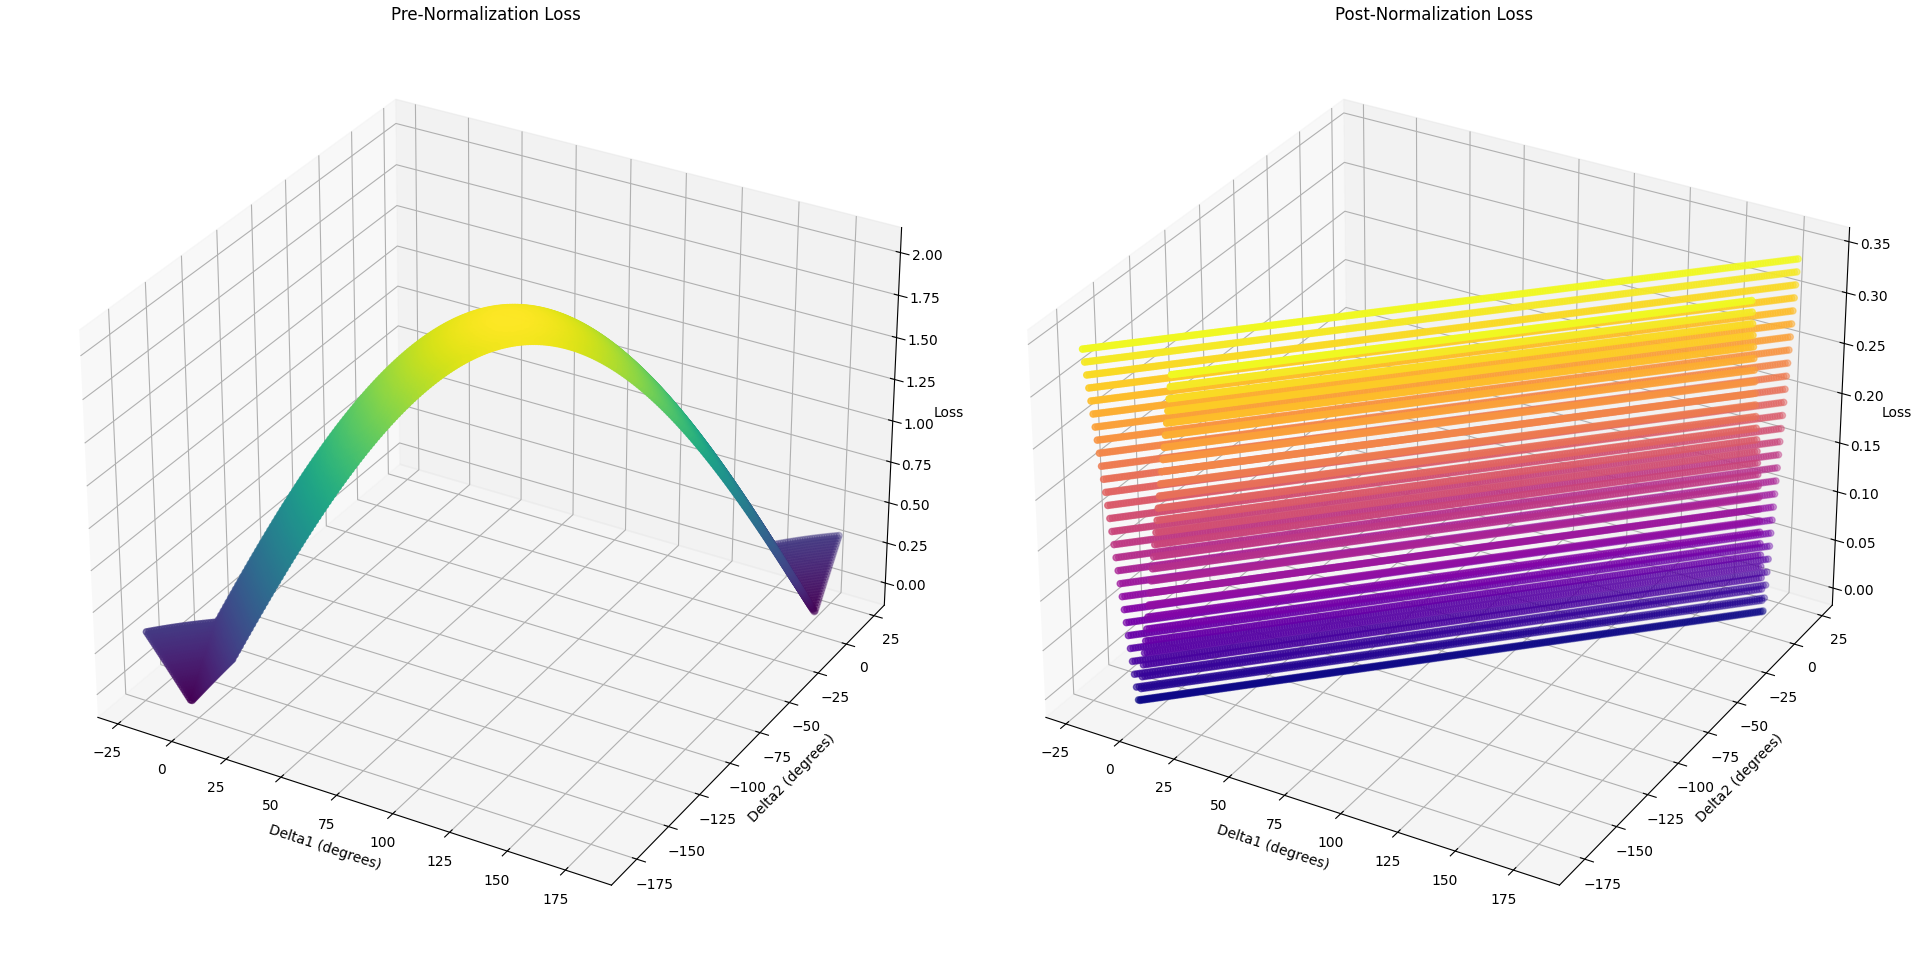
\includegraphics[width=\textwidth]{Chapter 4/Figs4/lossprevspost.png}
    \caption{Loss comparison between pre-normalization and post-normalization methods.}
    \label{fig:lossprevpost}
\end{figure}


As seen in Figure~\ref{fig:lossprevpost}, the pre-normalization method results in losses exceeding 2.0 due to the compounding effect of treating both images independently. In contrast, the post-normalization method, which works with relative rotation, consistently yields lower losses, with a maximum loss of approximately 0.35 under these typical UAV conditions. Therefore, post-normalization is expected to provide more accurate translation estimations due to better retention of keypoint information.




\subsubsection*{Empirical Validation}

In empirical tests, these results were confirmed, with post-normalization consistently providing higher accuracy due to better retention of keypoint information. The effects were most significant in the DESERT dataset, where the sparsity of keypoints made the dataset particularly sensitive to information loss during rotation. 

\subsubsection*{Method Conclusion}

Given the UAV's typical flight pattern and the need to minimize information loss, post-normalization is applied. In this approach, images are first aligned, followed by translation estimation. Finally, the translation vector is normalized to the global NE coordinate space for consistent navigation.




\section*{Image Similarity Computation}

In order to choose which image to infer location based on, the image with the highest similarity to the current image must be chosen. This is done by comparing the current image to all images in the database. The image with the highest similarity is then chosen.
To ensure this computation is efficient, a two-stage process is employed:
- Proximity search space reduction
- Similarity computation


\subsection*{Search Space Reduction}
This stage involves reducing the space to only images that the UAV could likely be close to. This is based on the UAV's last known location. However, a fixed radius is susceptible to errors if the frame rate or UAV speed is not fixed. As such, a dynamic search radius is employed, increasing until a certain number of images are found. 


\subsection*{Global Matching Techniques}

After initial search space reduction, a more accurate similarity computation is done for all potential image matches. Global techniques take the entire image as context to compute similarity. Its critical that this similarity estimation is efficient as multiple images will be compared. Further, to ensure matches are truly similar, the image context should be captured evenly across the image. 
Prior to similarity computation, images are rotated to be aligned together, as the global matching methods require. 


xxx - add in scope that no methods are used that require pre- or live-training.




\subsubsection*{Local detectors and matcher conversion techniques}
Retrofitting local matching techniques, which operate on keypoints, to a global matching context is done by computing the similarity using the amount of good matches between images. 
However, this does not guarantee an even distribution of matching across the image, leading to sub-par similarity computation. 
To combat this, grid matching is used, and a maximum number of matches is set per grid. This method is computationally expensive, but it is extremely robust to distortions and rotational changes. 
The most accurate, while still computationally efficient, detector and matcher are employed, ORB and FLANN, respectively. xxx check.


\subsubsection*{Cross-correlation}  
Cross-correlation measures the similarity between two images by sliding one over the other and calculating a sum of pixel-wise multiplications at each position. The maximum sum occurs when the two images are best aligned, indicating the point of greatest similarity. 

\subsubsection*{Histograms}  
Histograms compare images by analyzing the distribution of pixel intensities across a set of bins, typically 256 for an 8-bit image. Each bin represents a range of pixel intensities, and the method counts how many pixels fall into each bin. The comparison is performed by calculating the difference between the histograms of two images, often using metrics like Chi-Square or Bhattacharyya distance. This method is based on global color and brightness distributions, and not spatial shifts. 

\subsubsection*{SSIM (Structural Similarity Index)}  
SSIM compares two images by breaking down their similarities into three components: luminance, contrast, and structure. It first calculates the local means (for luminance), variances (for contrast), and covariances (for structure) over small windows. The similarity in luminance, contrast, and structure between corresponding windows is then measured and combined into a single score. SSIM is designed to model how humans perceive image quality, focusing on structural information like edges and textures.

\subsubsection*{Phase Correlation}  
Phase correlation is used to determine the similarity between two images by analyzing the confidence in a given maximum likelihood translational offset. It is similar to cross-correlation but operates in the frequency domain, where it uses only the phase information. This means it focuses on global structural as opposed to local ones, becoming robust to noise and illumination changes but losing some resolution. It also has a lower time complexity since it cross-correlation involves convolution (O($n^2$)) while phase correlation involves multiplication (O(nlogn)). 
To compare the images, the phase components are extracted and the cross-power spectrum is computed. This is done by multiplying the phase of one image by the complex conjugate of the phase of the other image, which effectively cancels out the magnitude information and highlights the phase differences. The result is then normalized to remove any bias introduced by varying magnitudes. After computing the cross-power spectrum, an inverse Fourier transform is applied to convert the result back into the spatial domain, where a sharp peak appears. The height and sharpness of this peak reflect the confidence of the match, while the position of the peak indicates the translational offset between the two images.
doesnt work well 




\subsubsection*{Hashing}  
Hashing provides a compact representation of an image by converting its pixel data into a fixed-size hash value, which simplifies comparison. In average hashing (for example), the image is resized, converted to grayscale, and the average pixel value is computed. Each pixel is compared to this average, and a binary string (hash) is generated by assigning 1s and 0s depending on whether the pixel value is above or below the average. Hashing is useful for quickly comparing images to detect similarities or duplicates, with differences measured via Hamming distance between the hash values. However, from empirical testing, hashing was found to be much less accurate than other methods, and was not further pursued.

\subsection*{}

\subsubsection*{Future Work}
In future, using a single image to infer location will be replaced by a more complex system that weights the estimate given by multiple images to infer location. Further, this will not increase runtime significantly. This method is not tested in this study, due to time constraints and the fact it is likely to make the solution too easy, without having to put much effort into the accuracy of the pipeline. xxx maybe ill test this out later. 


\section*{Translational Estimators}

Estimating the translation between two images is crucial, as it directly infers the GPS shift between frames. 
Prior to translation estimation, images and point clouds are aligned together. Empirical tests show that separating rotation and translation improves accuracy, even with methods designed to estimate both simultaneously. Estimating fewer transformations reduces the potential for errors, leading to more precise results.
After estimation, the translation values are aligned to the global heading space. 
Given the altitude of the UAV, the main transformations in the images are rotation and translation, with minor perspective distortions in some cases. 
Empirical tests show global matchers, which operate on the entire image, are much less robust, and have variances in estimations hundreds of times larger than local matchers. For this reason, local matchers are used for translation estimation.
xxx - this is also true for rotational estimators.
xxx- need to merge these



\subsection*{Primary Methods for Estimating Transformations}



\subsubsection*{Direct Source Normalization with Rotation Correction}
This method first normalizes the source and destination points by centering them around their means. It then uses Singular Value Decomposition (SVD) to estimate the rotation, correcting for any minor rotational discrepancies. The translation is calculated by averaging the differences between the aligned points.  
DoF: 3 (translation in x and y, and rotation). 

\subsubsection*{Affine Transformation with RANSAC}
Affine transformation, estimated via `cv2.estimateAffine2D`, captures translation, rotation, and scaling simultaneously. RANSAC is applied to filter outliers. While flexible, the combined estimation of multiple transformations may lead to less accurate translation estimates, as rotation and scaling adjustments may interfere with precise translation calculation.  
DoF: 6 (translation in x and y, rotation, scaling in x and y, shear).

\subsubsection*{Rigid Transformation Estimation (SVD)}
This method preserves the shape of the object by using SVD to estimate both rotation and translation. It first centers the points and then determines the rotation matrix, followed by the translation.  
DoF: 3 (translation in x and y, and rotation). 

\subsubsection*{Homography Transformation}
Homography estimates a transformation that maps points between two planes, capturing translation, rotation, scaling, and perspective distortion. It is estimated using `cv2.findHomography`.  
DoF: 8 (translation, rotation, scaling, and perspective changes in x and y).







% General 

feature detection dynamic optimization is fine bc it does not use prior kniowledge of the dataset, and is not far enough down the pipeline to force false positives into the dataset, it detects alot of keypoints and allows the future stages to deal with it. 


\section*{optimization Techniques}
Due to the large variance of optimal parameter sets as any prior pipeline method or parameter is varied, this set is only calculated once for the optimal pipeline. Further, the idea is not to get the absolute best value, as this depends on the dataset. The idea is to rather find a parameter that works well, and given the other stages being well-chosen, this crude parameter choice should work well without full optimization. More specifically, if the optimization stage only works well with highly tuned parameters, then the entire pipeline and task cannot be considered robust or generalizable.  
However, note that for the above tests, crude estimates for the most optimal parameter set per parameter set were used to ensure each method was tested under optimal conditions, and optimization techniques did not add bias to any specific methods. More specifically, optimization was applied to every technique and method above to ensure they were tested near their full potential. 

\subsubsection*{RANSAC for Affine Transformation}
RANSAC is used to improve the robustness of affine transformation estimation by iteratively selecting random subsets of points and fitting it to a model estimation like affine. This filters out outliers, ensuring only the most reliable matches contribute to the final transformation matrix. 
Its main parameter choice is a reprojected error threshold, which determines how far a point can be from the model to be considered an inlier. This method is extremely sensitive to the quality and number of keypoints found. This parameter WAS xxx. Using dynamic thresholding until a sufficient number of inliers were found, was not pursued, as it forces unatural matches into the dataset. That is, in sparse datasets it will force in false positives, and in dense datasets it will force out true positives. Since this is the final stage prior to the rotational and translational estimation, forcing false positives into the dataset will introduce massive errors. 

\subsection*{Lowe's Ratio Test}
Lowe's ratio test is used to filter matches based on the ratio of the best match's distance to the second-best match's distance. If the ratio is below a certain threshold, the match is retained. This test is crucial for removing ambiguous matches, ensuring only the most reliable correspondences are used for further processing. Lowe's ratio works on the basis that if a match is the best match, it should be sufficiently closer to the target keypoint than the second-best match. However, if it is not the best match, and is a false positive, then it is likely that the second-best match, also a false positive, is not significantly further, in descriptor space, from the target keypoint. Since almost every keypoint in the source image is matched with another keypoint in the destination image, there will be many false positives considering many matches are moved off the image as the UAV moves. If RANSAC was applied prior to this, many false positives would be included, and RANSACs model will be flooded with false positive, rendering it unable to find the correct model. This is why Lowe's ratio test is crucial. However, Lowe's ratio is also extremely sensitive to the number and quality of keypoints found. If there are very many keypoints relative to the ratio, correct matches might be removed due to the high number of keypoints implying a higher likelihood that the second-best match is very close in descriptor space. If Lowe's ratio is however too lenient it will allow through too many false positives. Dynamic thresholding was applied here. The aim was to minimize its impact, since it is somewhere in the middle of the pipeline so it does have a decent effect on the final estimation. Lowe's ratio was chosen such that it should ideally generalize well and only run once. However, if insufficient matches were found, the threshold is slowly made more lenient until a sufficient number of matches were found. This does run a risk of adding false positives into the dataset, however, it is necessary to ensure stability and enough matches are found in varying datasets. 


Empirical Testing Only:
Confidence based matching - threshold based on number of matches in sorted distance. This was not pursued as it was extremely sensitive to the number of keypoints found, and the quality of the keypoints. There is no way to know, for each dataset in general, how many good matches there are. This forces a number which might work well for one dataset, but completely fail for another. It runs the main risk of removing too many good matches.
absolute thrseholding matches: This was based on absolute distance thresholding. ie there has to be an absolute closeness thrsehold met between the two kps in descriptor space. However, it was seen in empirical tests to be redundant given Lowe's ratio accounts for this implicitly, and it also led to instability, ie no effect or too few matches. The above number of matches is more robust. However, the above still not great bc xyz. this one either had no effect, or negative. highly unstable across tested thresholds. 




